% These are the lecture notes for my CSC1101 course Fall 2016
% at CityTech. They are based largely on How To Think Like A
% Computer Scientist. See last slide for reference information.

% Feel free to edit these slides and use them for your own courses.
% Email me at: awood [at] citytech.cuny.edu
% or at: awood [at] gradcenter.cuny.edu


\documentclass{beamer}

\usepackage{tikz}
\usetikzlibrary{calc}

\usepackage{forest}
\usepackage{verbatim}
\usepackage{color}


\setbeamertemplate{footline}[frame number]
\setbeamertemplate{navigation symbols}{} 

\newtheorem{thm}{Theorem}[section]
\newtheorem{lem}{Lemma}
\newtheorem{cl}{Claim}
\newtheorem{cor}{Corollary}[section]
\newtheorem{conj}{Conjecture}
\newtheorem{quest}{Question}
\newtheorem{defn}{Definition}[section]
\newtheorem{obs}{Observation}[section]
\newtheorem{exam}{Example}

\newcommand{\im}{\operatorname{im}}
\newcommand{\id}{\operatorname{id}}
\newcommand{\interior}{\operatorname{int}}
\newcommand{\bdry}{\operatorname{bdry}}
\newcommand{\<}{\langle}
\renewcommand{\>}{\rangle}
\newcommand{\Gab}{(G_\phi)^{ab}} 
\newcommand{\phibar}{\bar{\phi}}
\newcommand{\Z}{\mathbb{Z}}
\newcommand{\N}{\mathbb{N}}
\newcommand{\Q}{\mathbb{Q}}
\newcommand{\R}{\mathbb{R}}
\newcommand{\C}{\mathbb{C}}
\newcommand{\A}{\mathcal{A}}
\newcommand{\OO}{\mathcal{O}}
\newcommand{\UU}{\mathcal{U}}
\newcommand{\power}{2^{\{P_1, \cdots , P_n\}}}
\newcommand{\bp}{\begin{problem}}
\newcommand{\ep}{\end{problem}}
\newcommand{\ba}{\begin{answer}}
\newcommand{\ea}{\end{answer}}
\newcommand{\ds}{\displaystyle}
\newcommand{\ben}{\renewcommand{\theenumi}{\alph{enumi}}
\renewcommand{\labelenumi}{(\theenumi)}\begin{enumerate}}
\newcommand{\een}{\end{enumerate}}
\newcommand{\Hess}{\operatorname{Hessian}}
\newcommand{\Aut}{\mathrm{Aut}}
\newcommand{\Inn}{\mathrm{Inn}}
\newcommand{\Out}{\mathrm{Out}}
\newcommand{\End}{\mathrm{End}}


\mode<presentation>
{
%  \usetheme{default}
  \setbeamercovered{invisible}
}


\usepackage[english]{babel}
\usepackage[latin1]{inputenc}
\usepackage{times}
\usepackage[T1]{fontenc}
\usepackage{stmaryrd}

%\usetheme{default}
%\usetheme{AnnArbor}
%\usetheme{Antibes}
%\usetheme{Bergen}
%\usetheme{Berkeley}
%\usetheme{Berlin}
%\usetheme{Boadilla}
%\usetheme{CambridgeUS}
%\usetheme{Copenhagen}
%\usetheme{Darmstadt}
%\usetheme{Dresden}
%\usetheme{Frankfurt}
%\usetheme{Goettingen}
%\usetheme{Hannover}
%\usetheme{Ilmenau}
%\usetheme{JuanLesPins}
%\usetheme{Luebeck}
%\usetheme{Madrid}
%\usetheme{Malmoe}
%\usetheme{Marburg}
%\usetheme{Montpellier}
%\usetheme{PaloAlto}
%\usetheme{Pittsburgh}
%\usetheme{Rochester}
\usetheme{Singapore}
%\usetheme{Szeged}
%\usetheme{Warsaw}

%\usecolortheme{default}
%\usecolortheme{albatross}
\usecolortheme{beaver}
%\usecolortheme{beetle}
%\usecolortheme{crane}
%\usecolortheme{dolphin}
%\usecolortheme{dove} % grey, white, yellow
%\usecolortheme{fly} %grey, yellow
%\usecolortheme{lily} %white, yellow, blue
%\usecolortheme{orchid}
%\usecolortheme{rose}
%\usecolortheme{seagull}
%\usecolortheme{seahorse}
%\usecolortheme{whale}
%\usecolortheme{wolverine}

% Title page

\title[Intro to Python]{Introduction to Python}

\subtitle{IDLE and Python 2.7}

\author
{Lecture notes of Alexander Wood \\ \scriptsize \href{mailto:awood@citytech.cuny.edu}{awood@citytech.cuny.edu}}
\institute[CityTech]{New York City College of Technology }  

\date{}

\begin{document}

\begin{frame}
  \titlepage
\end{frame}



\section{What is a program?}


%%%%%%%%%%
\begin{frame}
\frametitle{What is a program?}

A \textbf{program} consists of instructions that specify how to perform some task. There are many types of tasks a program can perform: 
\begin{itemize}
\item Mathematical computation
	\begin{itemize}
	\item Solving systems of equations
	\end{itemize}
\item Symbolic computation
	\begin{itemize}
	\item Finding all instances of a word in a text document
	\end{itemize}
\item Graphical computation
	\begin{itemize}
	\item Image recognition
	\item Playing videos online
	\end{itemize}
\end{itemize}
\end{frame}

%%%%%%%
\begin{frame}
\frametitle{Input and Output}

Many programs take \textbf{input} and/or yield some \textbf{output}.

\begin{itemize}
\item
\textbf{Input:} Get data from the user, from a file, etc.
\item \textbf{Output:} Print data, save data in a file, etc.
\end{itemize}
\end{frame}

%%%%%%%%
\begin{frame}[fragile]
\frametitle{Program Flow}

We utilize various code structures to control which lines of code execute.

\begin{itemize}
\item\textbf{Conditional execution:} Evaluate certain code blocks under certain conditions. For instance, \verb|if| and \verb|else| statements.
\item\textbf{Repetition Structures:} Repeat some action.
\end{itemize}
\end{frame}



\section{Running Python}

\begin{frame}[fragile]
\frametitle{Running Python}

\begin{itemize}
\item You can run Python from your browser 
	\begin{itemize}
	\item PythonAnywhere
	\end{itemize}
\item  The Python interpreter
	\begin{itemize}
	\item Accessed by typing \verb|python| or \verb|python3|  from command line
	\end{itemize}
\item IDLE, an integrated development environment
\end{itemize}
\end{frame}


\section{IDLE}


\begin{frame}
\frametitle{IDLE}
IDLE combines: 

\begin{itemize}
\item Interactive Python shell
\item Color-coding text editor
\item ``Check module" for syntax errors
\item Search tools
\item Text formatting for auto-indentation
\item Debugger tool
\end{itemize}
\end{frame}

\begin{frame}
\frametitle{Opening IDLE}

\begin{itemize}
\item Mac: Go to applications, select the Python folder, and double-click ``IDLE"
\item PC: Select Python from Start menu, select ``IDLE"
\end{itemize}
\centering
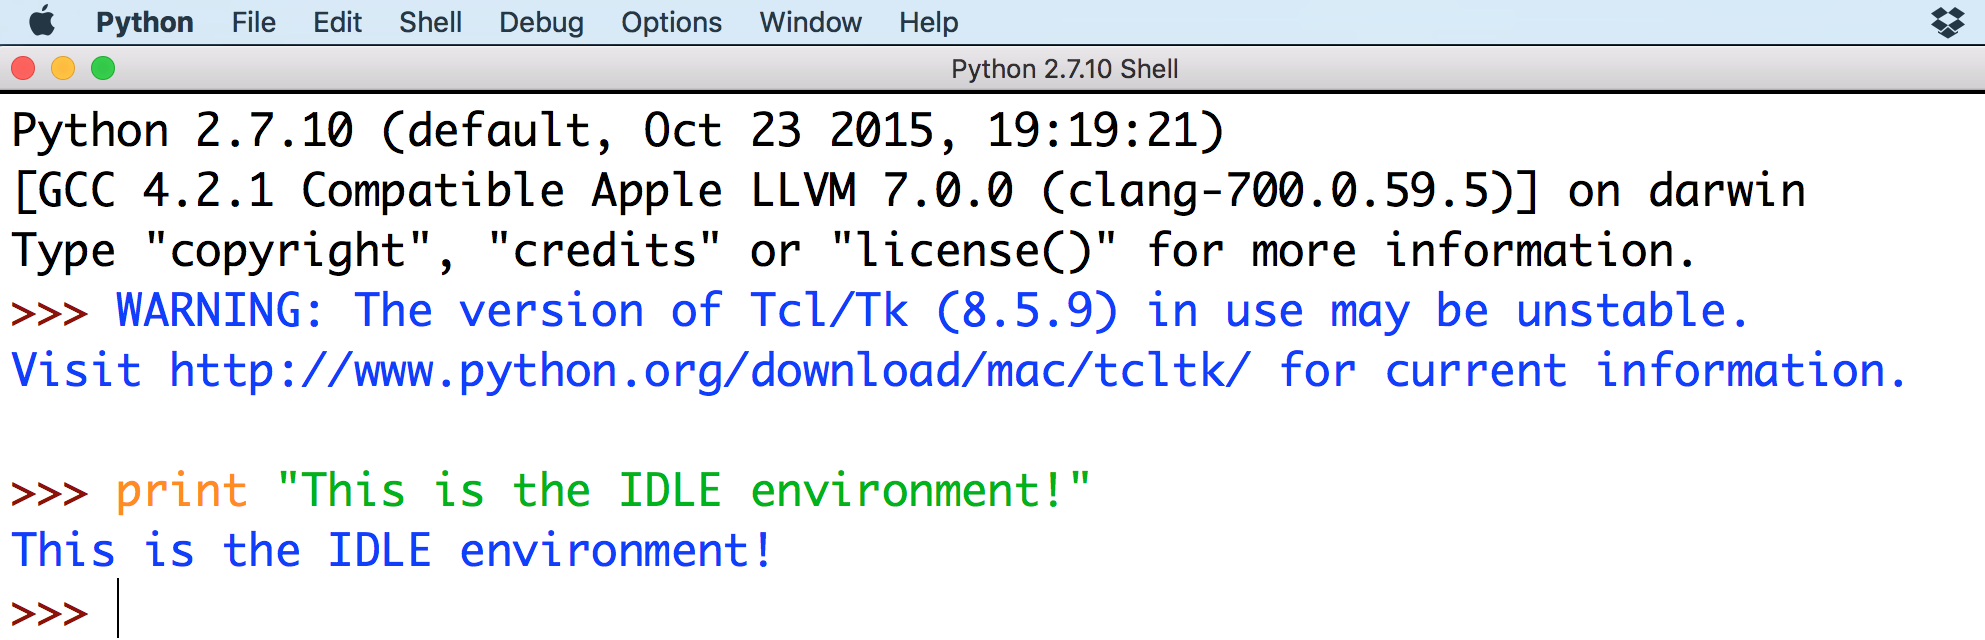
\includegraphics[scale=.3]{IMG/1idle.png}
\end{frame}




%%%%%%%%%%
\begin{frame}[fragile]
\frametitle{Using IDLE}

The \verb|>>>| prompt indicates that you may write a Python statement. When you press \verb|Enter|, the statement is executed.
\begin{figure}
\centering
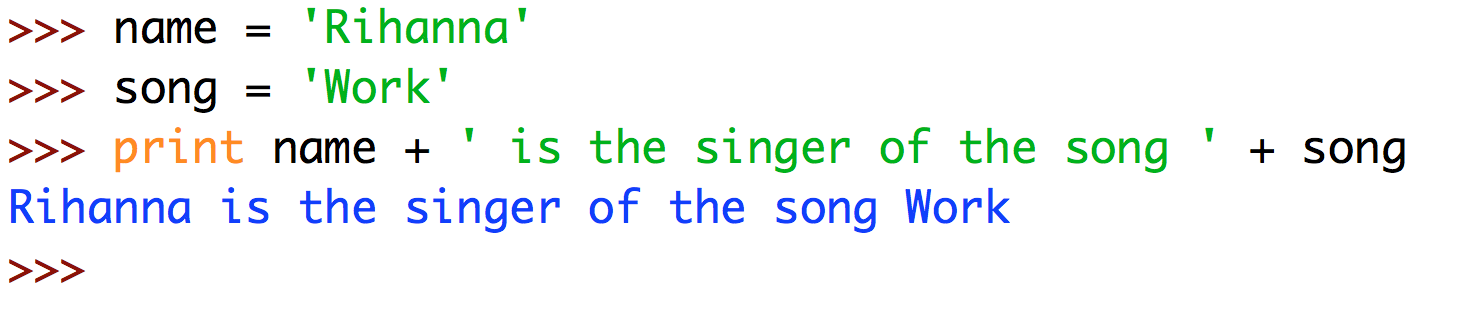
\includegraphics[scale=.4]{IMG/2idle.png}
\end{figure}
\end{frame}


%%%%%%%%%%
\begin{frame}
\frametitle{Using IDLE: Multiline statements}

Multiline statements in IDLE:

\begin{figure}
\centering
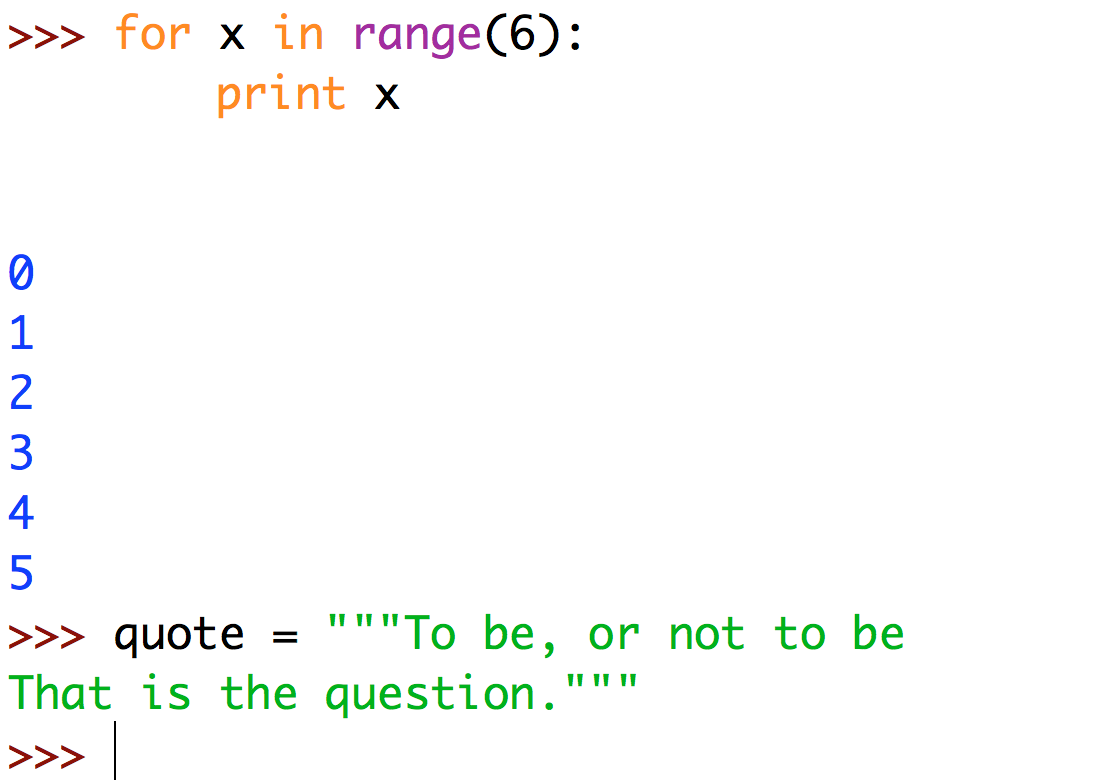
\includegraphics[scale=.3]{IMG/3idle.png}
\end{figure}
\end{frame}


%%%%%%%%%%
\begin{frame}
\frametitle{Writing a Python program using IDLE}

Open a new editing window

\begin{figure}
\centering
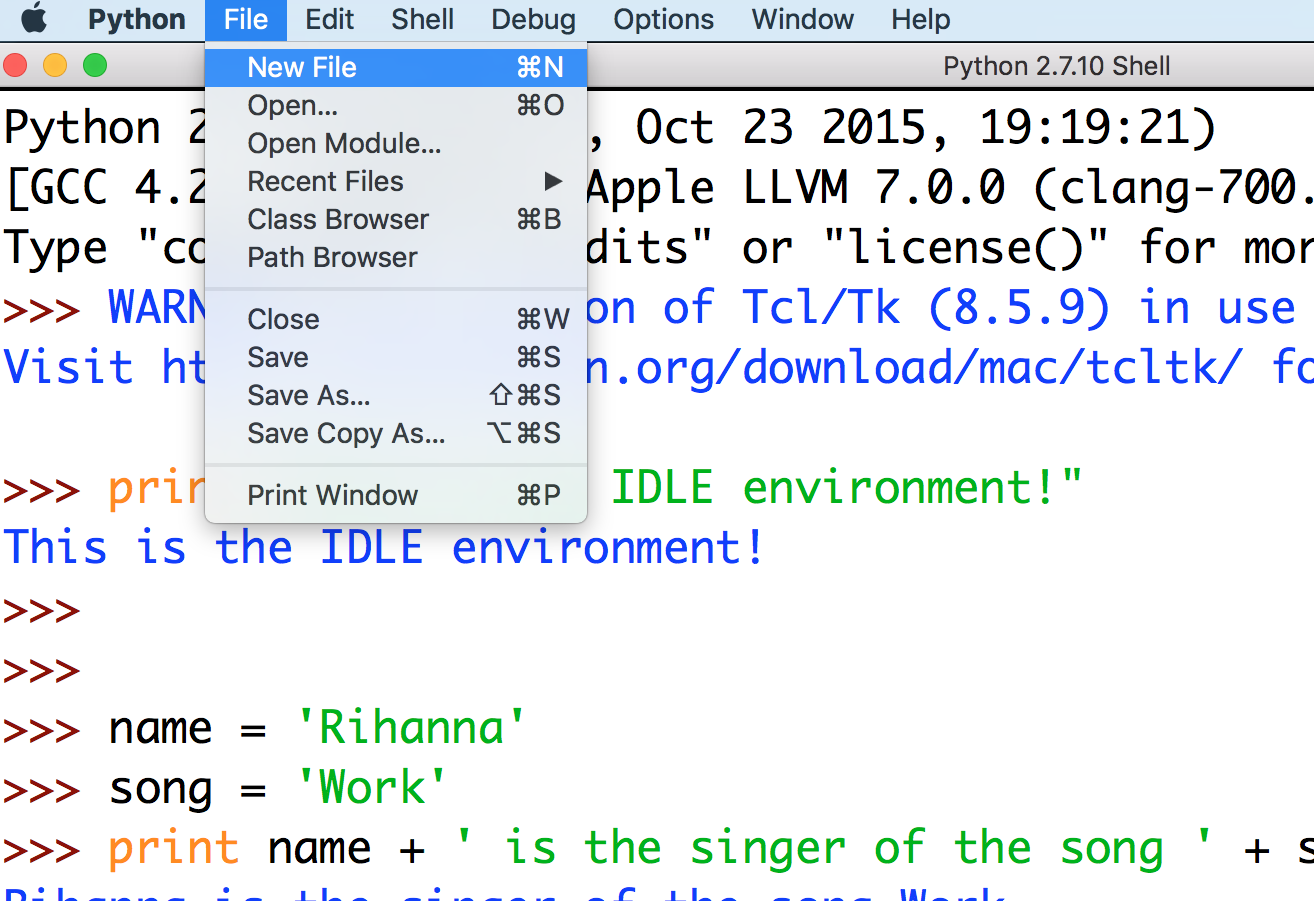
\includegraphics[scale=.4]{IMG/4idle.png}
\end{figure}
\end{frame}





%%%%%%%%%%
\begin{frame}
\frametitle{Example Program in IDLE}

\begin{figure}
\centering
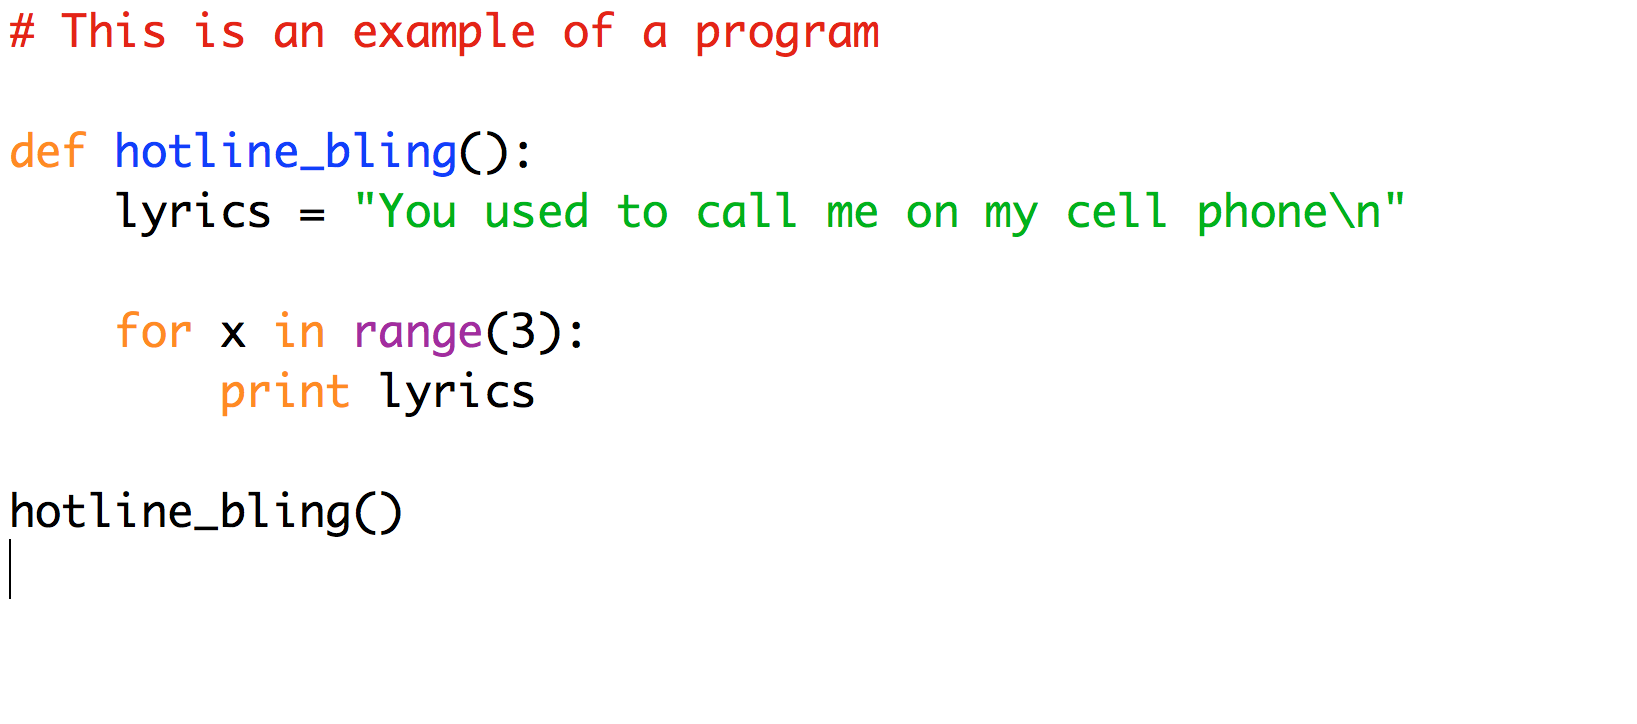
\includegraphics[scale=.4]{IMG/5idle.png}
\end{figure}
\end{frame}

\begin{frame}
\frametitle{Color Coding in IDLE}

\begin{itemize}
\item \color{blue} \textbf{Blue:} Defined names, such as functions and classes
\item \color{orange} \textbf{Orange:} Python keywords
\item \color{red} \textbf{Red:} comments
\item \color{green} \textbf{Green:} String literals
\item \color{purple} \textbf{Purple:} Built-in functions
\item \color{black} \textbf{Black:} Everything else!
\end{itemize}
\end{frame}



%%%%%%%%%%
\begin{frame}
\frametitle{Running the test program in IDLE}

\begin{itemize}
\item First, save the program!  
\item Second, press F5 or Run > Run Module
\end{itemize}
\begin{figure}
\centering
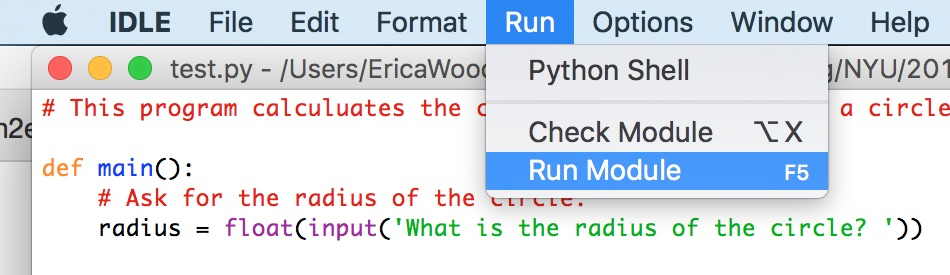
\includegraphics[scale=.2]{IMG/6idle.jpg}
\end{figure}
\end{frame}



%%%%%%%%%%
\begin{frame}
\frametitle{Running the test program in IDLE}

The program then runs in IDLE's Python Shell.

\begin{figure}
\centering
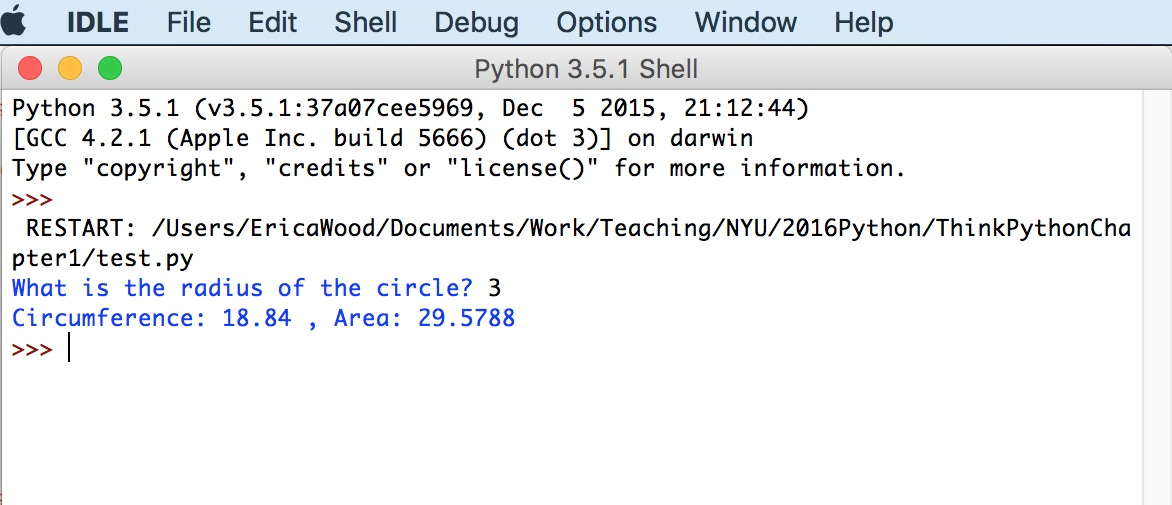
\includegraphics[scale=.2]{IMG/7idle.jpg}
\end{figure}

\end{frame}


\section{Snakehandling}
\begin{frame}
\frametitle{Two Modes of Python}

\begin{itemize}
\item \textbf{Interactive mode} is using python interactively, by typing directly into the python interpreter. Open up IDLE and type away!
\item \textbf{Python Programming}, is programming in the python language, where .py scripts are run.
\end{itemize}
\end{frame}


\section{Expressions}

\begin{frame}[fragile]
\frametitle{Expressions: Values and Types}

\begin{itemize}
\item \textbf{Value:} The basic building blocks of a program! For instance, a letter, or a number.
	\begin{itemize}
	\item Examples: \verb|42|, \verb|3.14|, \verb|'hotline bling'|
	\end{itemize}
\item \textbf{Type:} Every value belongs to a specific type. For instance, 
	\begin{itemize}
	\item \verb|42| is an \verb|int|, \verb|3.14| is a \verb|float|, and \verb|'hotline bling'| is a \verb|string|.
	\end{itemize}
\end{itemize}
\end{frame}

\begin{frame}[fragile]
\frametitle{Data Types}

A few data types available in Python are:
\begin{itemize}
\item \textbf{Booleans}, which take value \verb|True| or \verb|False|
\item \textbf{Integers}, whole numbers
\item \textbf{Floats}, numbers with decimals
\item \textbf{Strings}, sequences of text characters
\end{itemize}
\end{frame}

\begin{frame}[fragile]
\frametitle{Determining Types}

Determine the type of a value by calling the built in function \verb|type()|

\begin{figure}
\centering
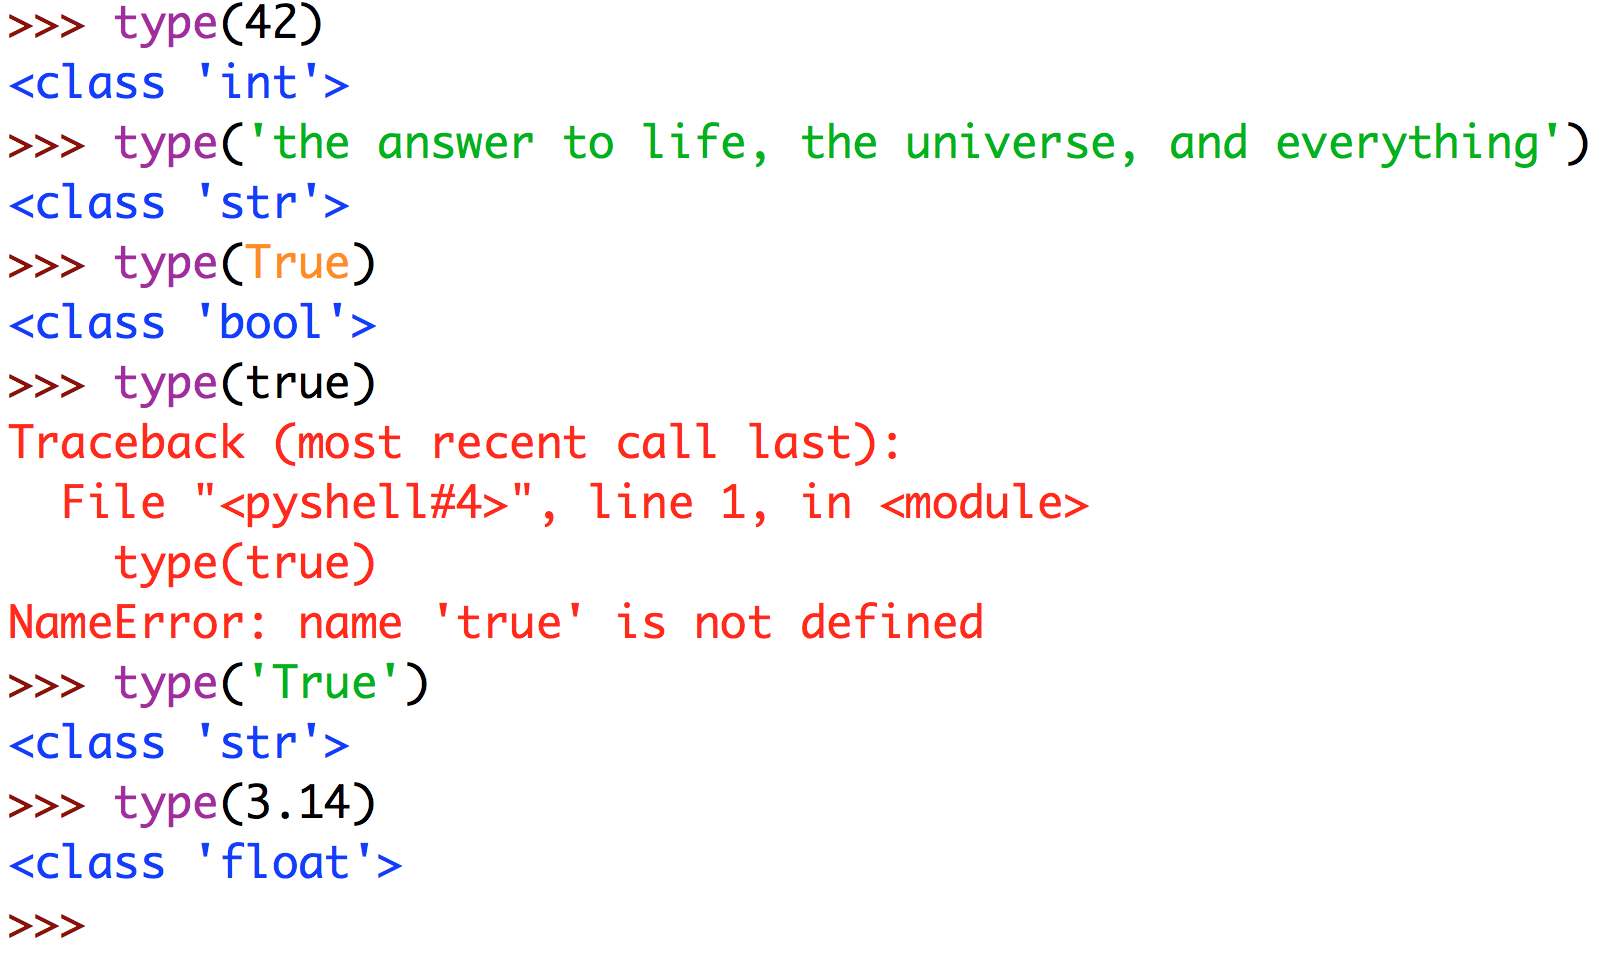
\includegraphics[scale=.3]{IMG/type.png}
\end{figure}
\end{frame}


\section{Debugging}

\begin{frame}
\frametitle{Debugging}

When you make a mistake in your code, you will receive an error. These errors are called \textbf{bug}. Getting rid of the bugs in your code is called \textbf{debugging}. Sometimes the mistake is as simple as a misspelled word, whereas other times the error is in the code structure itself. Tracking down bugs can be time-consuming and stressful, and it is important to learn various debugging skills. We will discuss various techniques throughout the course.
\end{frame}

\section{2.x VS 3.x}

\begin{frame}[fragile]
\frametitle{Python 2.x VS Python 3.x}

\begin{itemize}
\item Python $3$ is backwards incompatible with Python $2$ and introduces new features.
\item \verb|print| is a function in Python 3 but a statement in python 2
\item For more information on the differences see \url{https://docs.python.org/3.1/whatsnew/3.0.html}
\end{itemize}
\end{frame}

\section{References}

\begin{frame}
\frametitle{References}

\begin{itemize}
\item
How to think like a computer scientist: Learning with Python, chapter 1
\url{http://www.openbookproject.net/thinkcs/python/english2e/ch01.html}

\item
Official Python  2 documentation
\url{https://docs.python.org/2/}
\end{itemize}
\end{frame}
\end{document}


